%% Research framework (simple overview). Compile with pdflatex.
\documentclass[tikz,border=1pt]{standalone}
\usepackage{amsmath}
\usepackage{txfonts}
\usetikzlibrary{arrows.meta,positioning,calc}
\newcommand{\bW}{\mathbf{W}}
\definecolor{cD}{HTML}{3F4B5B}\definecolor{cX}{HTML}{1F5A8C}\definecolor{cE}{HTML}{2E7040}
\definecolor{cT}{HTML}{A33B36}\definecolor{cO}{HTML}{5A3F8A}\definecolor{cP}{HTML}{A0601C}
\definecolor{cWire}{HTML}{3A3A42}
\begin{document}
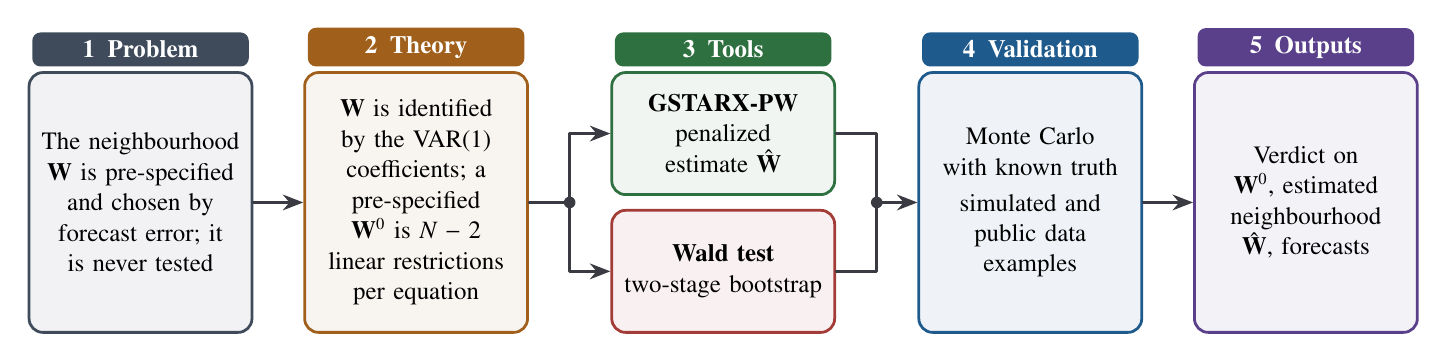
\begin{tikzpicture}[
  font=\rmfamily\small, line cap=round, line join=round,
  >={Stealth[length=2.6mm,width=2.0mm]},
  box/.style={draw=#1, fill=#1!7!white, line width=1pt, rounded corners=5pt, minimum height=3.3cm,
              text width=2.55cm, align=center, inner sep=4pt,
              execute at begin node={\hyphenpenalty=10000\exhyphenpenalty=10000}},
  head/.style={fill=#1, text=white, font=\rmfamily\bfseries\small, rounded corners=3pt, inner sep=3pt,
               minimum width=2.75cm, align=center},
  wire/.style={draw=cWire, line width=1pt},
  arr/.style={wire, ->},
  dot/.style={circle, fill=cWire, inner sep=0pt, minimum size=4.2pt},
]
\def\xA{0}\def\xB{3.5}\def\xC{7.4}\def\xD{11.3}\def\xE{14.8}
\def\jL{5.45}\def\jR{9.35}
\node[box=cD] (b1) at (\xA,0) {The neighbourhood $\bW$ is pre-specified and chosen by forecast error; it is never tested};
\node[box=cP] (b2) at (\xB,0) {$\bW$ is identified by the VAR(1) coefficients; a pre-specified $\bW^0$ is $N-2$ linear restrictions per equation};
\node[box=cE, minimum height=1.55cm] (b3a) at (\xC,0.875) {\textbf{GSTARX-PW}\\ penalized estimate $\hat{\bW}$};
\node[box=cT, minimum height=1.55cm] (b3b) at (\xC,-0.875) {\textbf{Wald test}\\ two-stage bootstrap};
\node[box=cX] (b4) at (\xD,0) {Monte Carlo with known truth\\[2pt] simulated and public data examples};
\node[box=cO] (b5) at (\xE,0) {Verdict on $\bW^0$, estimated neighbourhood $\hat{\bW}$, forecasts};
\node[head=cD, anchor=south] at (\xA,1.72) {1\enspace Problem};
\node[head=cP, anchor=south] at (\xB,1.72) {2\enspace Theory};
\node[head=cE, anchor=south] at (\xC,1.72) {3\enspace Tools};
\node[head=cX, anchor=south] at (\xD,1.72) {4\enspace Validation};
\node[head=cO, anchor=south] at (\xE,1.72) {5\enspace Outputs};
\draw[arr] (b1.east) -- (b2.west);
\draw[wire] (b2.east) -- (\jL,0);
\draw[arr] (\jL,0) |- (b3a.west);
\draw[arr] (\jL,0) |- (b3b.west);
\draw[wire] (b3a.east) -| (\jR,0);
\draw[wire] (b3b.east) -| (\jR,0);
\draw[arr] (\jR,0) -- (b4.west);
\draw[arr] (b4.east) -- (b5.west);
\node[dot] at (\jL,0) {};
\node[dot] at (\jR,0) {};
\end{tikzpicture}
\end{document}
